
\chapter{Methods for Learning Depth and Visual Odometry from Light Fields}

In Chapter 3, we saw that previous work has produced a variety of approaches to depth estimation and visual odometry, using both data-driven and hand crafted solutions. In this chapter, a pipeline is presented that matches the pipelines seen in chapter 3 in appearance, but differs in the functionality and type of input data. The contributions of previous work focus on the use of monocular and stereo image data, while this chapter focuses on developing a pipeline that employs the full breadth of geometric information in a light field. The first section of this chapter describes the tools and methodologies of acquiring a suitable dataset, while the second part walks through the development of the pipeline used.

\section{Data Acquisition}

\subsection{Ground Truth Pose Data}

\begin{figure}[h]
    \centering 
    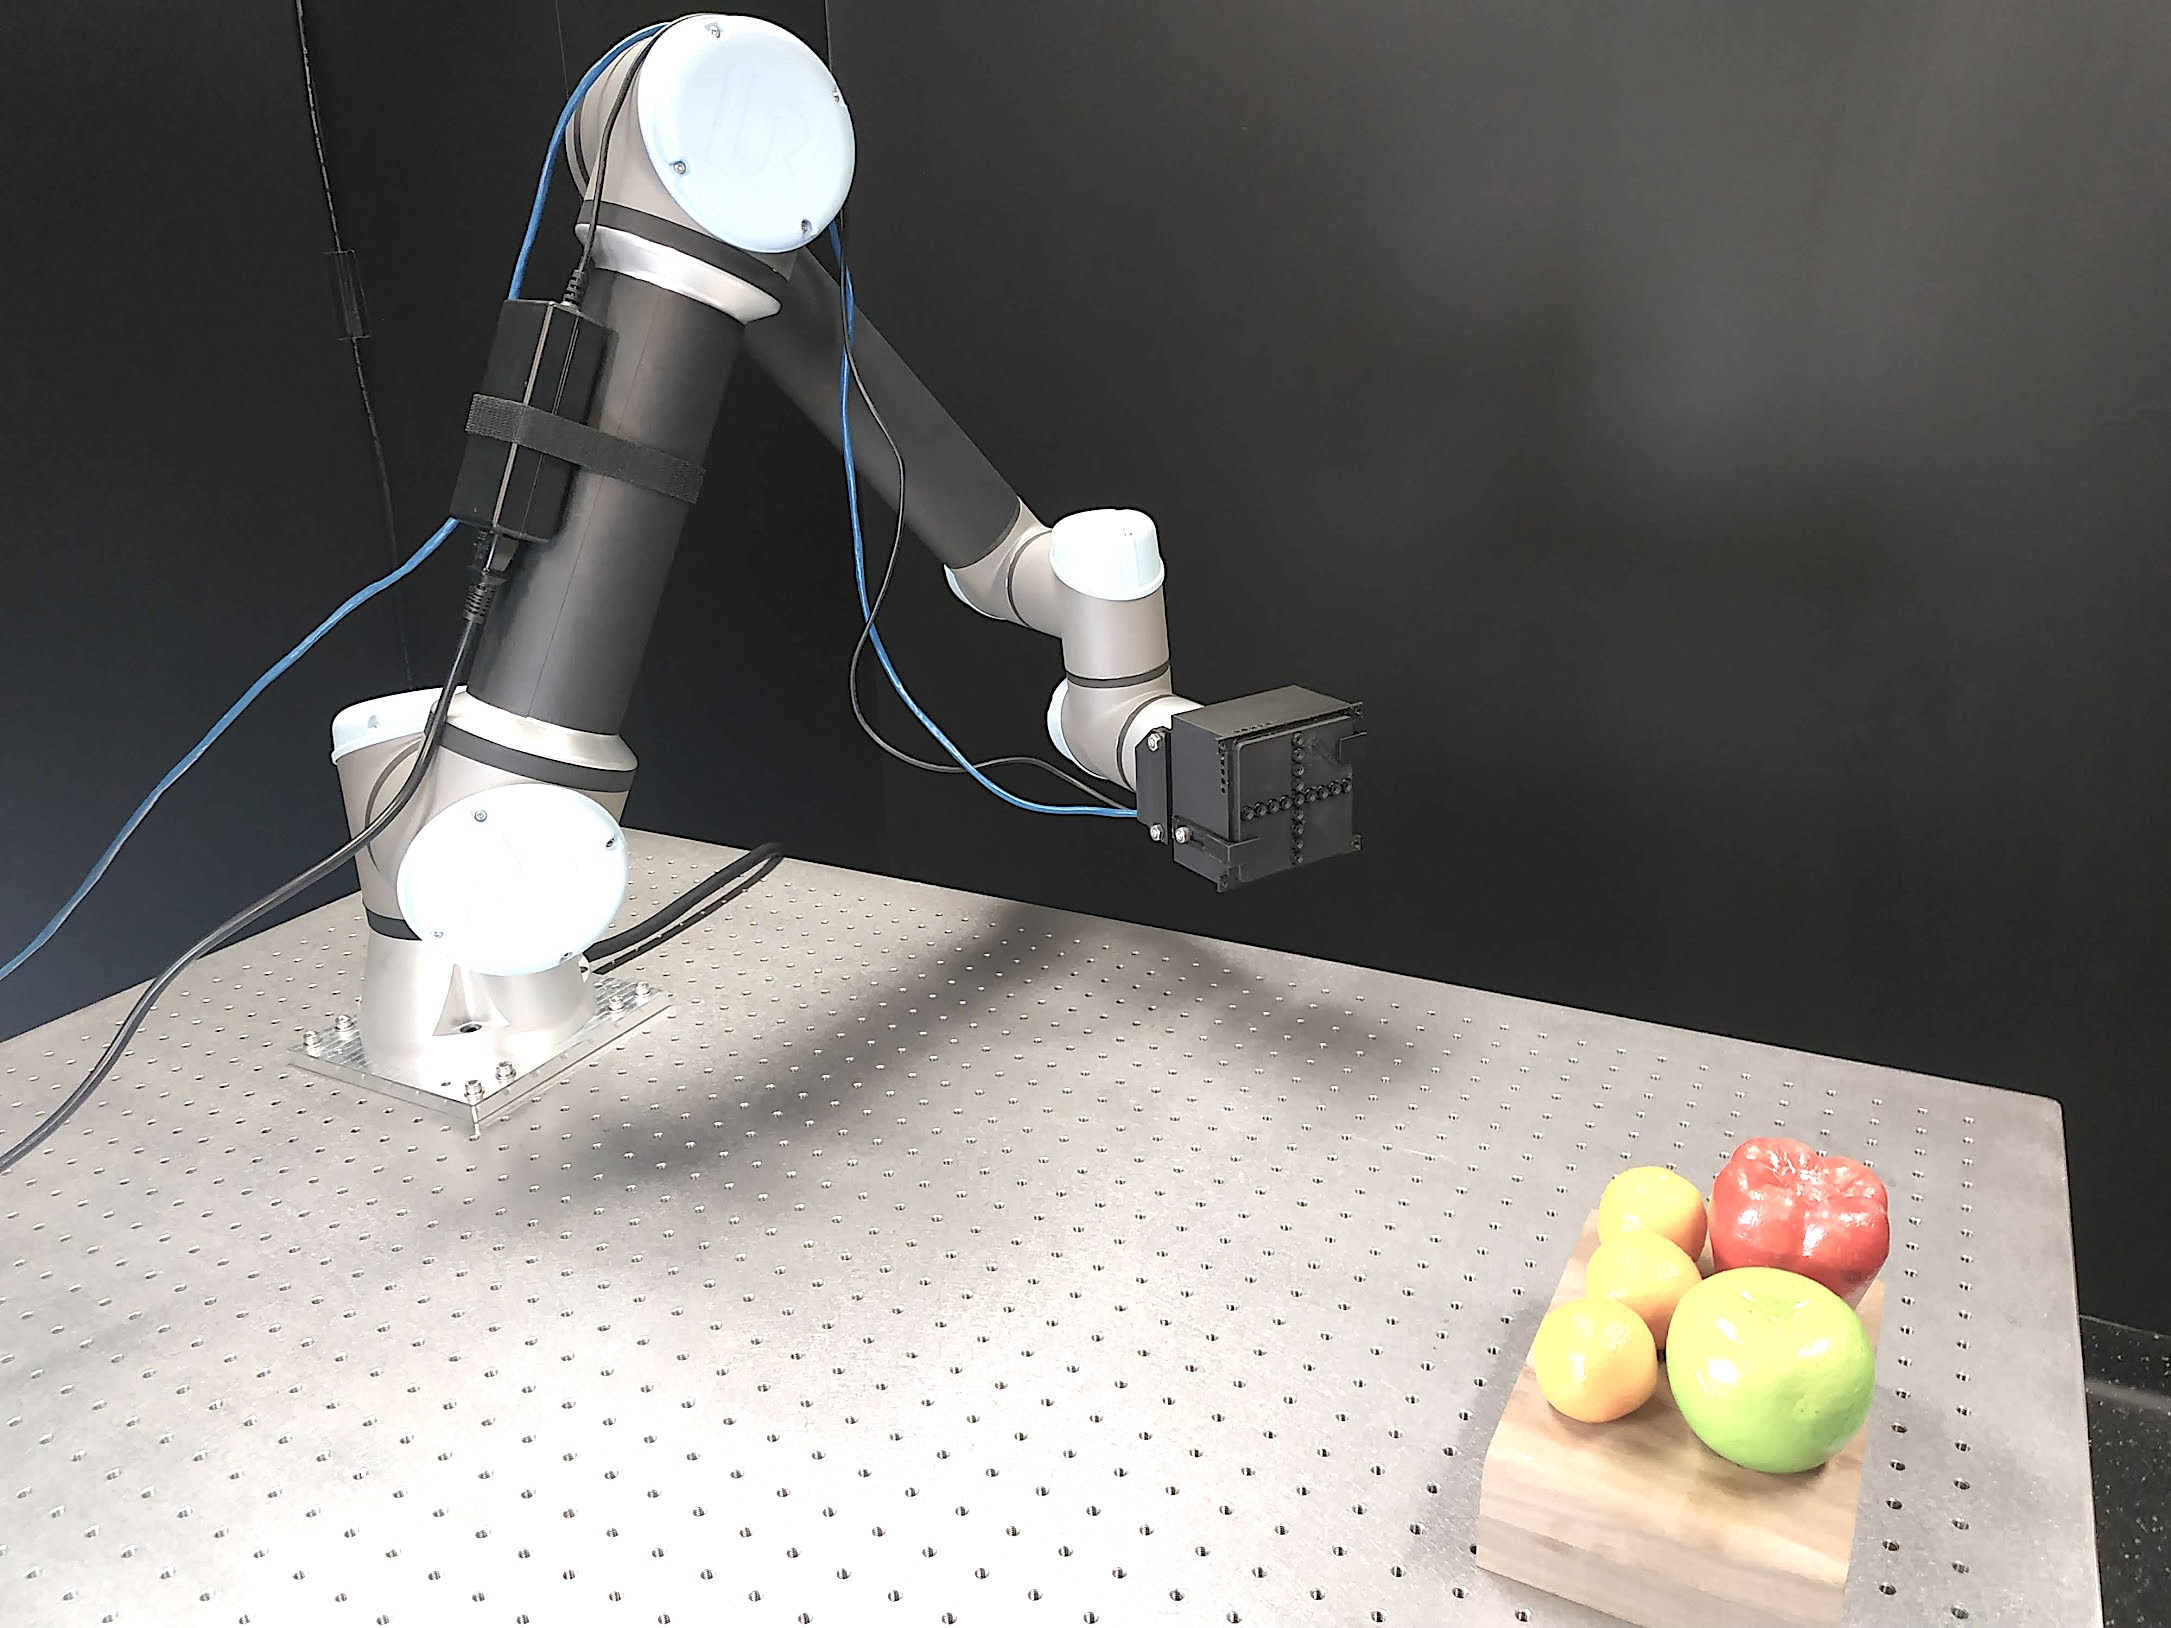
\includegraphics[width=4.5in]{images/experimentalsetup2.jpg}
    \caption{The experimental setup utilises a Universal Robots UR5E robotic arm to precisely measure ground-truth pose to allow effective evaluation of the projects visual odometry results.}
\end{figure}

Important to this work is a strong evaluation framework. Existing datasets such as KITTI and CityScapes benefit from state-of-the-art sensor suites including inertial sensors and lidar, allowing researchers to effectively benchmark their results. Similarly, this thesis places a strong emphasis on validation using ground truth data. One of the primary tasks for evaluation is visual odometry, and so ground-truth pose data for each image is a valuable resource. In this project, pose is collected by attaching the camera to a Universal Robots UR5E robotic arm, which is capable of sensing to a high degree of accuracy the pose of the end effector. Furthermore, the UR5E is able to perform accurate movements and trajectories with payloads of up to 5 kilograms, making it a suitable robotic mount for the camera. 

A challenge that needed to be solved prior to data collection was thus fabricating a rig for attaching the camera to the end effector. The UR5E uses a standard interface plate for attaching end-effectors such as grippers and other tools. The camera on the other hand, as an early prototype, does not have any suitable mounts available on the market for attaching it to the robot. A suitable mount therefore needed to be fabricated, taking into consideration the cameras ventilation and electronic connection requirements. A two-piece mount was designed using SolidWorks, and fabricated using fused deposition modelling (FDM) with polylactic acid (PLA) filament, allowing easy mounting and dismounting to the robot using standard M6 bolts. 

A client library for communicating with the UR5E was written in python, which establishes a TCP/IP connection with the robot over the local network, allowing both movement commands to be sent to the robot, and feedback data about the end-effector's pose to be streamed back to the client PC. The client library also provides functionality for pre-computing trajectories and joint angles, using the PyBullet physics engine and the known kinematic model of the robot. One useful trajectory function from the client library procedurally generates new waypoints with a stringent collision-checking mechanism, meaning data-collection can be performed autonomously. A challenge that has prevented a fully autonomous footage collection routine has been working with non-timestamped image data. The particular imaging setup currently provides only enough bandwidth for image data at roughly 1 frame every 2 seconds. Furthermore, the onboard rectification processes take several seconds to complete, and what's more, because the on board storage of the camera is limited, the image must be streamed over an ethernet connection to a PC taking several more seconds. The actual time that the image is captured is therefore ambiguous and so correlating each image with a pose-stamp is difficult. An intermediate solution has been to manually control the arm to each waypoint, and pausing while an image is taken and the pose is saved. 

\subsection{Imagery}

The specific imaging device being used is manufactured by EPIImaging, and consists of 17 subapertures. The communication interface with the camera is a network connection serving image data over the HTTP protocol via a straightforward URL request. Both rectified and unrectified images can be requested, and the format of the returned image data is a $17\times 3 \times 1280 \times 960$ block of bytes representing pixel data from each of the 17 image sensors. A simple client library was written in python that automates the URL request, and subsequent decoding of image bytes, allowing data to be collected quickly and conveniently.


\section{Depth and Visual Odometry Pipeline}

\begin{figure}[htbp]
    \centering 
    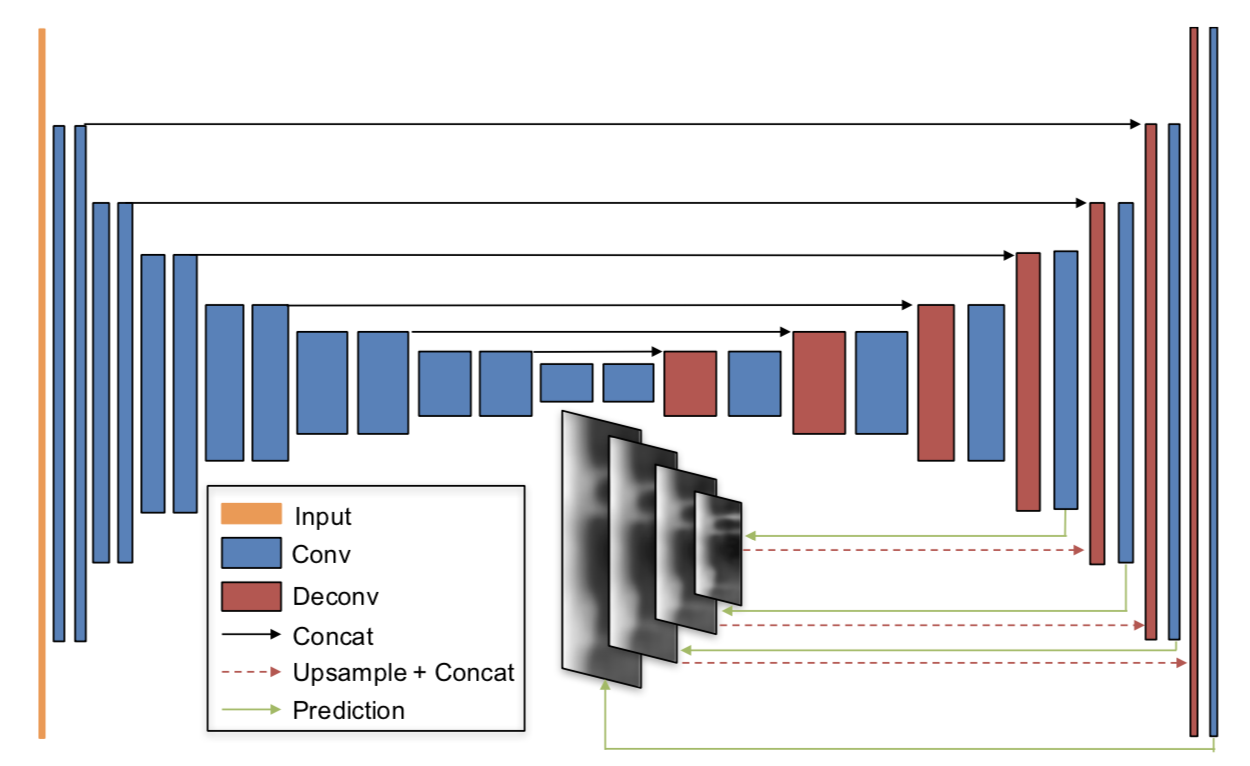
\includegraphics[width=2.5in]{images/dispnet.png}
    
\includegraphics[width=0.5in]{images/blank.png}
    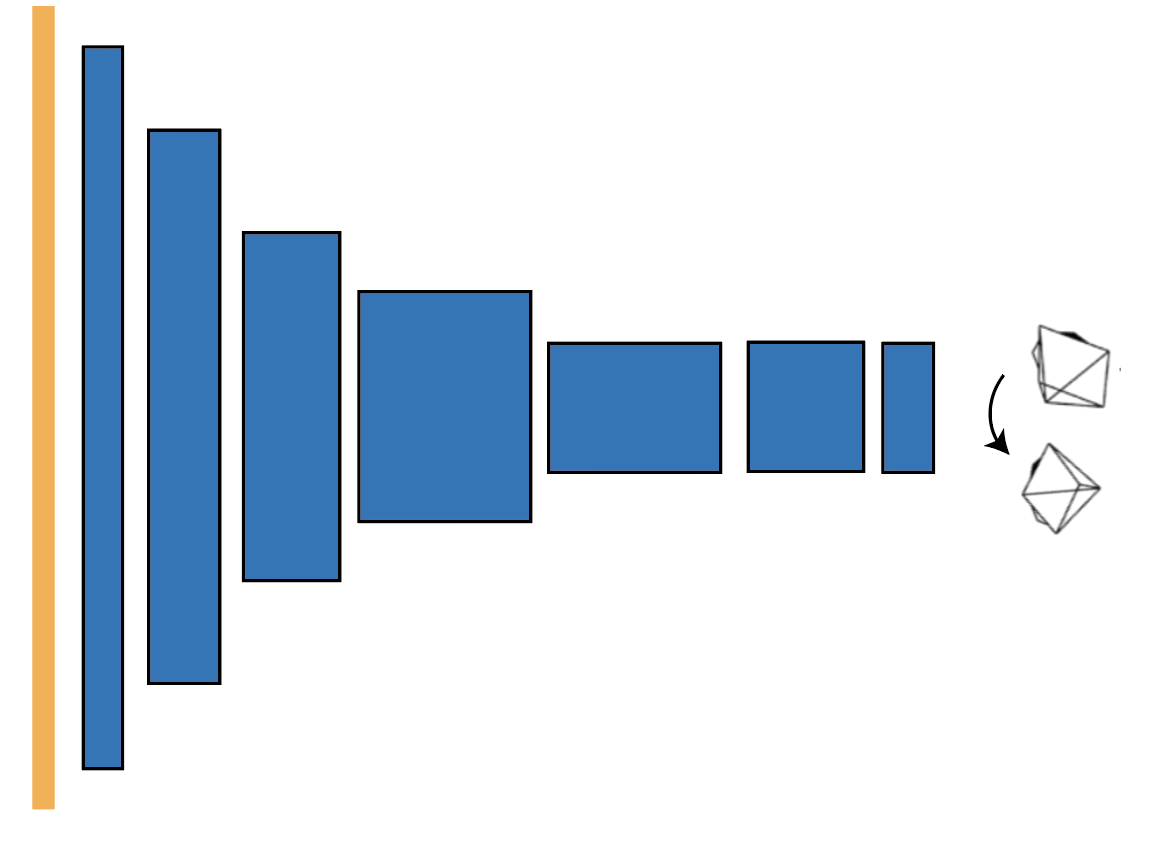
\includegraphics[width=2in]{images/posenet.png}
    \caption{(Left) The DispNet architecture uses a convolution encoder-decoder network characterised by skip connections, and outputs predictions at multiple scales. The multi-scale predictions aid in handling low-texture regions of the image. (Right) The PoseNet architecture uses a series of convolutional downsampling operations, predicting a final 6 degree-of-freedom pose estimate at its output activations.}
 \end{figure}

\subsection{Pose Estimation}

Estimating the 6-degree-of-freedom pose between two frames is treated as a regression problem, estimating three translational components [X, Y, Z] and three rotational components [Rx, Ry, Rz]. Importantly, the translation and rotation are regressed relative to the \textit{camera} coordinate frame of the first image, whereas the UR5E returns absolute position and orientation in the \textit{world} coordinate frame. The data preprocessing pipeline is thus required to compute the relative translation $P_{t1 \rightarrow t2}$ and rotation $R_{t1 \rightarrow t2}$ of two images, given their absolute positions $P_{t1}, P_{t2}$ and orientation $R_{t1}, R_{t2}$ in world coordinates. Concatenating translation and rotation into a single transform matrix $T = [R|t]$ allows us compute both relative rotation and translation in a single step, as:

\begin{equation}
T_{t1 \rightarrow t2} = T_1^{-1} T_2.
\end{equation}

The transform matrix can subsequently be decomposed into 3 translational and 3 rotational components. 

Regression of pose values is done with a CNN. As described in Chapter 2, there have been a variety of methods proposed for feeding light field images to CNNs. As of now, experiments have been conducted using light fields formatted as a stack of images concatenated along their colour channels. The two light fields are subsequently fed to the CNN, which produces 6 output values corresponding to the 6 degrees of freedom. The 'rectified linear unit' non-linearity function (ReLU) is used as an activation layer following each convolutional layer except the output prediction layer. 


\subsection{Depth Estimation}

Depth estimation is similarly modeled as a regression problem, with the same number of outputs as inputs. The depth estimation module uses a convolutional encoder-decoder architecture called DispNet as proposed in \cite{mayer2015dispnet}. Skip connections from the encoder to the decoder mean the decoding layers are able to access both high level features and low level features on either side of the latent space.

% \begin{figure}[htbp]
%     \centering 
%     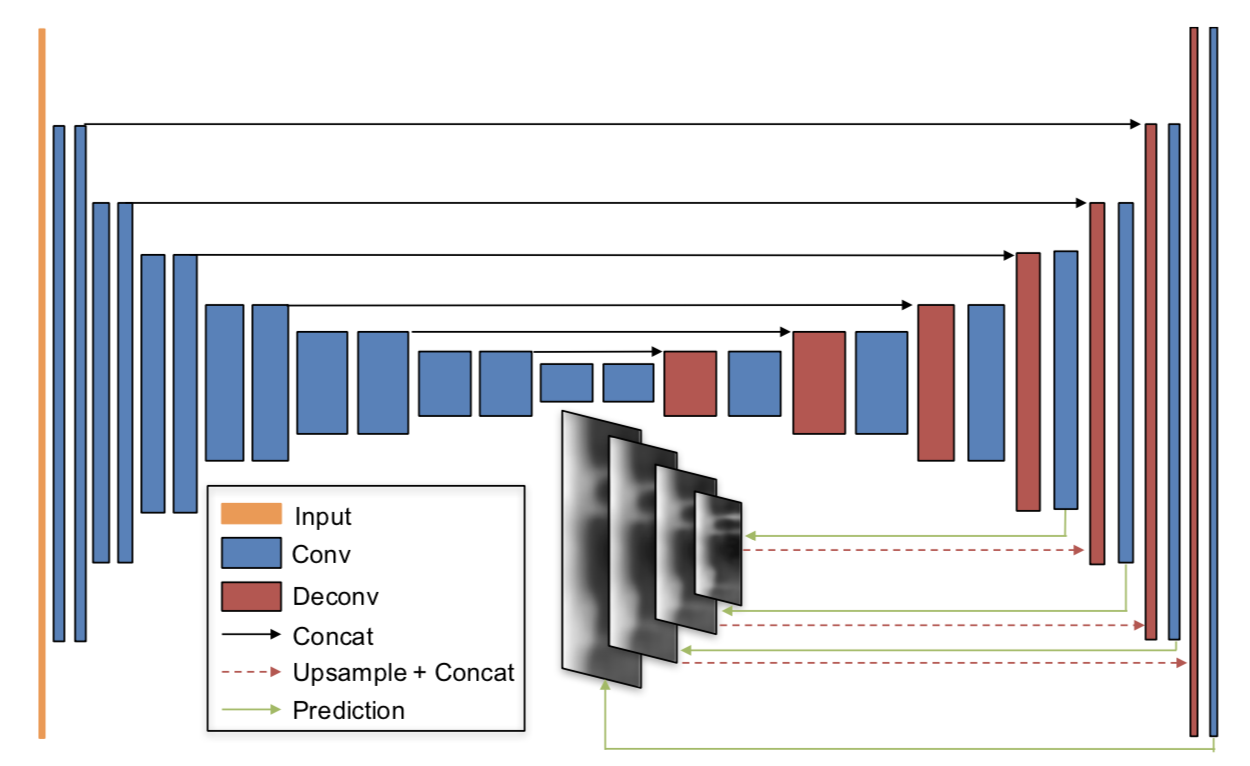
\includegraphics[width=3in]{images/dispnet.png}

%     \caption{The DispNet architecture uses a convolution encoder-decoder network characterised by skip connections, and outputs predictions at multiple scales. The multi-scale predictions aid in handling low-texture regions of the image.}
%  \end{figure}




\subsection{Differentiable Image Based Rendering}

Using the outputs from the depth and pose estimation modules, bilinear interpolation is used to photometrically reconstruct the first light field from the second. As described in Chapter 3, the procedure for this is to first project each pixel from $LF_1$ to a 3D point cloud using the known camera intrinsics and estimated depth values. Picking a single pixel $p1 = [s,t,u_1,v_1,1]^T$ from the first light field, and its corresponding depth estimate $D(p1)$, its projected point in 3D space is

\begin{equation}
    Q_{p1} = D(p1) K^{-1}[u_1,v_1,1]^T.
\end{equation}

The 3D coordinate $Q_{p1}$ can then be projected onto the camera sensor of $LF_2$, at the pixel coordinate $p_2 = [s,t,u_2,v_2]$. This relies on knowing the rigid transform $[R|t]$ from the first to the second camera origin.

\begin{equation}
    p_2 = K[R|t]Q_p.
 \end{equation}

This transform is equivalent to asking the question: knowing the depth of a pixel in image 1, where is the equivalent pixel in image 2? This procedure can be repeated for every pixel, allowing image 1 to be reconstructed entirely from the pixels of image 2. However, because pixels have discrete coordinates, and because we might find that the procedure described in equations 4.2 - 4.3 does not always produce an integer coordinate, the actual pixel value needs to be interpolated. The bilinear sampling kernel described in equations 3.3 - 3.5 is used as a differentiable method that supports backpropagation of errors. 

The supervision signal for the network is the sum of the photometric reconstruction loss (equation 3.1), and the regularising edge-aware smoothness loss (equation 3.2)

\begin{equation}
    L = L_{photometric} + L_{smooth}.
\end{equation}



\section{Experiments: Supervised Visual Odometry}

A simple, yet revealing experiment is to train a model to perform visual odometry in a fully supervised setting. While unsupervised methods form a supervision signal by cleverly piecing together the available information, a fully supervised approach on the other hand theoretically produces the best possible results for any given system. Thus, there is a motivation to test the performance of the neural architectures described above. Not only does this experiment uncover what the pose network is capable of, but the experiment lays the groundwork for future unsupervised experiments. Individual modules such as the network itself, the data-loading module and even the weights of the trained network \footnote{While using pretrained weights to reduce training time is common practice, care is taken in this work to avoid using overlapping datasets when using pretrained weights. The dataset used to supervise the pre-trained weights should not contain the same scenes used to train the unsupervised model.} can be reused in future experiments. 

\subsection{Monocular Visual Odometry}

In the first iteration of this experiment, the KITTI dataset is used thanks to the size of the dataset and the availability of ground truth pose measurements. The input to the network is the pair of images in the sequence, and the loss function is computed from the ground truth 6-degree-of-freedom pose transform from one frame to the next. Evaluation is performed on sequences of the KITTI dataset that were withheld at training time, so as to gain an understanding of the models ability to generalise outside of the training data. 

The network was trained for 18 hours, completing 70 passes over the input dataset. Stochastic gradient descent was used as the optimisation algorithm, using batch sizes of 8 images. The network was trained with pairs of image in both forwards and reverse order, meaning the network had to learn to predict both forwards and backwards motion. Input images were normalised with a mean pixel value at zero over the entire dataset, and divided by the standard deviation of the dataset. 


\begin{figure}[htbp]
    \centering
    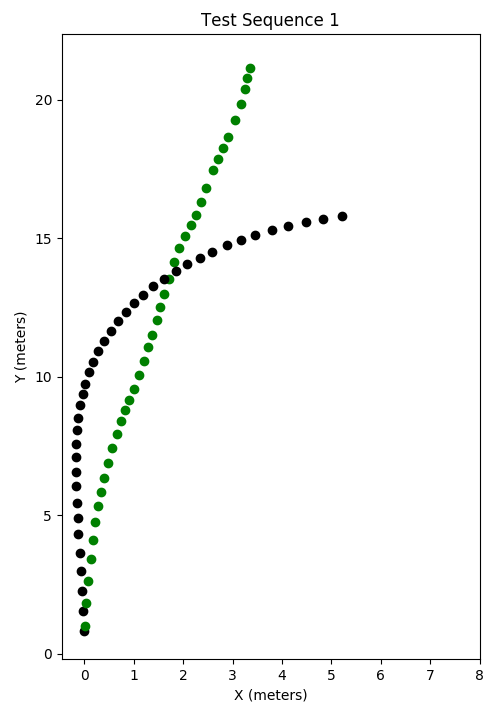
\includegraphics[height=2.4in]{images/vo_results/0034.png}
    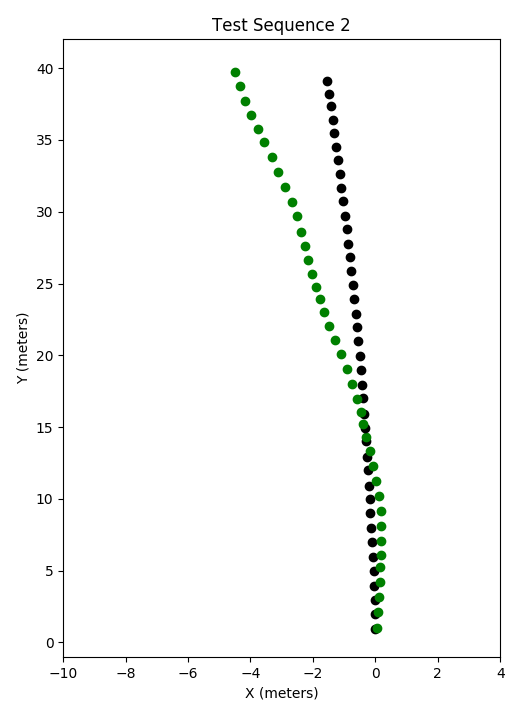
\includegraphics[height=2.4in]{images/vo_results/0018.png}
    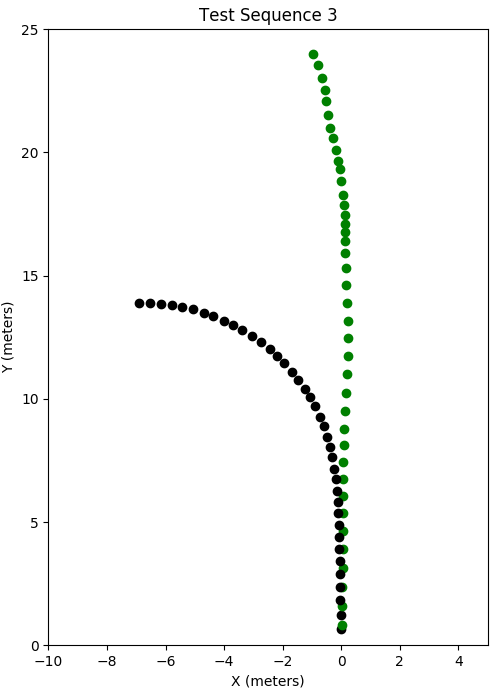
\includegraphics[height=2.4in]{images/vo_results/0027.png}
    
\includegraphics[height=0.2in]{images/vo_results/legend.png}

    \caption{Examples of trajectories generated from ground truth and estimated poses. These trajectories are generated over snippets of 40 frames from three test sequences which were withheld during training of the model. The cumulative nature of the error becomes more apparent the further the vehicle strays from the origin.}

    \label{vo_results_kitti}
    
\end{figure}

\begin{table}[tbp]

    \caption{Summary of Results for three test sequences}
    \centering
    \begin{tabular}{@{}llll@{}}
        \toprule
        Measure            & Sequence 1    & Sequence 2   & Sequence 3  \\ \midrule
        Frames             & 40            & 40           & 40          \\
        Path Length (m)    & 18.28         & 39.14        & 17.58       \\ \midrule
        \multicolumn{4}{l}{Instantaneous Translational RMS Error (m)}   \\
        X                  & 0.129         & 0.101        & 0.181       \\
        Y                  & 0.013         & 0.034        & 0.018       \\
        Z                  & 0.193         & 0.081        & 0.277       \\ \midrule
        \multicolumn{4}{l}{Absolute Trajectory RMS Error (m)} \\
        X                  &  0.81         & 1.39         & 2.70        \\
        Y                  &  2.17         & 0.24         & 5.42        \\
        Z                  &  0.12         & 0.37         & 0.25        \\ \bottomrule
    
        \end{tabular}
        \label{kitti_vo_results_tabular}
    \end{table}



Some examples of trajectories generated using raw-ground truth data and the predicted trajectories over 40 frame snippets of video are shown in Figure \ref{vo_results_kitti}. Because the trajectory of a vehicle driving along a road can be described almost entirely by its movements in a 2D plane, these trajectories are plotted as such, ignoring the minor up and down motions of the vehicle. While the error grows and becomes more evident at larger distances from the origin, the individual frame-to-frame error is qualitatively small. In observing these trajectories, we also note that while the network appears to have modeled forward and linear motion quite well, rotation seems to have been left behind. 

Results from the experiment are reported in Table \ref{kitti_vo_results_tabular}. The table summarises the instantaneous translational errors from frame to frame as well as the absolute pose error of the cumulative trajectory. These errors are computed as the root-mean-square error of the distance between the predicted and ground truth poses for the 3 translation components. In this table, instantaneous translational errors are reported relative to the X-Y-Z coordinate frame of the camera (Z pointing out through the lens), while the absolute trajectory error is reported relative to the coordinate frames shown in Figure \ref{vo_results_kitti}.







We observe in the tabulated results that the pose prediction consistently performs best in predicting translation in the $Z$ direction (up and down relative to the road). This is expected, as a vehicle driving on a flat road is likely to experience minimal up-and-down motion relative to the forwards-backwards and side-to-side components. The $Z$ translation of the cost function can thus be minimised easily by consistently predicting zero, or very close to zero for that component. Forwards and backwards instantaneous translations were predicted best in sequence two - a relatively straight stretch of road. This is indicative of the models difficulty when faced with tight corners as shown in sequences 1 and 3. 

\subsection{Plenoptic Visual Odometry}
A seemingly simple extension of the experiment described in the previous section is to perform the same procedure using light field imagery. With improved exposure to depth information, the model should see an improvement in performance, particularly in the awareness of scale. By providing multiple views, the model is able to implicitly learn the geometric features associated with the unchanging baseline between sub-apertures. This will aid in accurately predicting the magnitude of the rotations and translations in space. Such a model can learn to employ more robust features such as parallax and occlusion to estimate motion with improved scale awareness. After all, in the monocular case, the model must learn to infer scale from features of the scene (height above the ground or knowledge of the rough size of pedestrians could be features used by the model to make its predictions). 

While the pose network is capable of ingesting light field imagery and a small dataset is ready for training with, experiments thus far have yielded numerically unstable training losses, even in the case of single sub-apertures - an effectively identical approach to the experiment described in the previous section. An investigation is currently underway into the reasons behind this instability. ß